%% LyX 2.1.4 created this file.  For more info, see http://www.lyx.org/.
%% Do not edit unless you really know what you are doing.
\documentclass[a4paper,oneside,brazil,11pt,a4paper,openright,titlepage,usenames,dvipsnames]{book}
\usepackage[utf8]{inputenc}
\usepackage[T1]{fontenc}
\usepackage{lmodern}
\setcounter{secnumdepth}{3}
\setcounter{tocdepth}{3}
\usepackage{array}
\usepackage{verbatim}
\usepackage{calc}
\usepackage{textcomp}
\usepackage{amssymb}
\usepackage{graphicx}

\makeatletter

%%%%%%%%%%%%%%%%%%%%%%%%%%%%%% LyX specific LaTeX commands.
\pdfpageheight\paperheight
\pdfpagewidth\paperwidth

%% Because html converters don't know tabularnewline
\providecommand{\tabularnewline}{\\}

%%%%%%%%%%%%%%%%%%%%%%%%%%%%%% User specified LaTeX commands.
% Classe alternativa, apropriada para impressão frente-verso. Inclui páginas em branco
% de forma que capítulos sempre tenham início na página à direita:
% \documentclass[11pt,a4paper,openright,titlepage]{book}

% Pacotes
\usepackage[T1]{fontenc}
\usepackage[brazilian]{babel}
\usepackage{epsfig}
\usepackage{subfigure}
\usepackage{amsfonts}
\usepackage{amsmath}
\usepackage[thmmarks,amsmath]{ntheorem}%\usepackage{amsthm}
\usepackage{boxedminipage}
\usepackage{geometry}
\usepackage{theorem}
\usepackage{fancybox}
\usepackage{fancyhdr}
\usepackage{ifthen}
\usepackage{url}
\usepackage{afterpage}
\usepackage{color}
\usepackage{colortbl}
\usepackage{rotating}
\usepackage{makeidx}
\usepackage{indentfirst}
% Pacotes para adição de figuras do inkscape
\usepackage{graphicx}
\usepackage{import}

% Escolher um dos seguintes formatos:
\usepackage{ft2unb} % segue padrão de fontes do Latex

\makeindex

\makeatother

\usepackage{babel}
\begin{document}
\setcounter{secnumdepth}{3}
\setcounter{tocdepth}{2}
\pagestyle{empty}

\grau{Engenheiro de Controle e Automação}

\tipodemonografia{TRABALHO DE GRADUAÇÃO}

\begin{comment}
Título
\end{comment}


\titulolinhai{TÍTULO DO TRABALHO DIVIDIDO EM}

\titulolinhaii{MAIS DE UMA LINHA PARA TÍTULOS}

\titulolinhaiii{REALMENTE LONGOS COMO ESTE}

\titulolinhaiv{}

\begin{comment}
Autores. Basta retirar o texto totalmente caso não haja um determinado
autor.
\end{comment}


\autori{Rafael Lima}

\autorii{}

\autoriii{}

\begin{comment}
Membros da banca. Basta retirar o texto totalmente caso não haja um
determinado membro da banca.
\end{comment}


\membrodabancai{Prof. Fulano de Sousa, ENE/UnB}

\membrodabancaifuncao{Orientador}

\membrodabancaii{Prof. Ciclano dos Santos, ENE/UnB}

\membrodabancaiifuncao{Examinador interno}

\membrodabancaiii{Prof. Beltrano da Silva, ENE/UnB}

\membrodabancaiiifuncao{Examinador interno}

\membrodabancaiv{}

\membrodabancaivfuncao{}

\membrodabancav{}

\membrodabancavfuncao{}

\begin{comment}
Data de defesa: mês e ano
\end{comment}


\mes{Setembro}
\ano{\the\year}

\begin{comment}
Comandos para criar a capa e a página de assinaturas
\end{comment}


\capaprincipal
\capaassinaturas

\begin{comment}
Ficha Catalográfica
\end{comment}


\noindent \textbf{FICHA CATALOGRÁFICA}

\noindent %
\fbox{\begin{minipage}[t]{1\columnwidth}%
JOÃO, DA SILVA

Título do trabalho dividido em mais de uma linha para títulos realmente
longos como este,

\medskip{}


{[}Distrito Federal{]} 2015.

\medskip{}


x, 101p., 297 mm (FT/UnB, Engenheiro, Controle e Automação, 2015).
Trabalho de Graduação \textendash{} Universidade de Brasília.Faculdade
de Tecnologia.

\medskip{}


1. Bla\hfill{}2.Ble\hfill{}

3. Bli

\medskip{}


I. Mecatrônica/FT/UnB\hfill{}II. Título (Série)\hfill{}

%
\end{minipage}}

\noindent \medskip{}


\noindent \textbf{REFERÊNCIA BIBLIOGRÁFICA}

SILVA, JOÃO DA, (2015). Título do trabalho dividido em mais de uma
linha para títulos realmente longos como este. Trabalho de Graduação
em Engenharia de Controle e Automação, Publicação FT.TG-$n^{\circ}022$,
Faculdade de Tecnologia, Universidade de Brasília, Brasília, DF, 101p.

\noindent \bigskip{}


\noindent \textbf{CESSÃO DE DIREITOS}

\noindent AUTOR: João da Silva

TÍTULO DO TRABALHO DE GRADUAÇÃO: Título do trabalho dividido em mais
de uma linha para títulos realmente longos como este.

\noindent \medskip{}


\noindent GRAU: Engenheiro\hfill{}ANO: 2015\hfill{}

\noindent \medskip{}


É concedida à Universidade de Brasília permissão para reproduzir cópias
deste Trabalho de Graduação e para emprestar ou vender tais cópias
somente para propósitos acadêmicos e científicos. O autor reserva
outros direitos de publicação e nenhuma parte desse Trabalho de Graduação
pode ser reproduzida sem autorização por escrito do autor.

\noindent \bigskip{}


\noindent \rule[0.5ex]{1\columnwidth}{1pt}

\noindent João da Silva

\noindent Rua dos Bobos, nº 0, Bairro Feliz.

\noindent 71000-000 Brasília \textendash{} DF \textendash{} Brasil.


\begin{comment}
Dedicatória
\end{comment}


\frontmatter

\begin{comment}
Texto de dedicatória do primeiro autor.
\end{comment}


\dedicatoriaautori{um beijo pra minha mãe, pro meu pai, e pra você}

\begin{comment}
Texto de dedicatória do segundo autor. Caso não tenha um segundo autor,
este texto não será mostrado
\end{comment}


\dedicatoriaautorii{Dedicatória do autor 2}

\begin{comment}
Texto de dedicatória do terceiro autor. Caso não tenha um terceiro
autor, este texto não será mostrado
\end{comment}


\dedicatoriaautoriii{Dedicatória do autor 3}

\begin{comment}
Comando para criar a página de dedicatória
\end{comment}


\dedicatoria

\begin{comment}
Agradecimentos
\end{comment}


\begin{comment}
Texto de agradecimentos do primeiro autor.
\end{comment}


\agradecimentosautori{Agradecimentos!}

\begin{comment}
Texto de agradecimentos do segundo autor. Caso não tenha um segundo
autor, este texto não será mostrado.
\end{comment}


\agradecimentosautorii{A inclusão desta seção de agradecimentos é
opcional e fica à critério do(s) autor(es), que caso deseje(em) inclui-la
deverá(ão) utilizar este espaço, seguindo esta formatação.}

\begin{comment}
Texto de agradecimentos do terceiro autor. Caso não tenha um terceiro
autor, este texto não será mostrado.
\end{comment}


\agradecimentosautoriii{A inclusão desta seção de agradecimentos
é opcional e fica à critério do(s) autor(es), que caso deseje(em)
inclui-la deverá(ão) utilizar este espaço, seguindo esta formatação.}

\begin{comment}
Comando para criar a página de agradecimentos
\end{comment}


\agradecimentos

\resumo{resumo}{Resumo!

\medskip{}


Palavras Chave: bla, ble, bli

}\vspace*{2cm}


\resumo{Abstract}{Abstract, in English ofc!

\medskip{}


Keywords: bla, ble, bli

}

\begin{comment}
Listas de conteúdo, figuras e tabelas
\end{comment}


\sumario
\listadefiguras
\listadetabelas

\begin{comment}
Lista de Símbolos
\end{comment}


%TCIDATA{LaTeXparent=0,0,these.tex}


%\chapter*{\setfontarial\mdseries LISTA DE SÍMBOLOS} % se usar ft1unb.sty, descomente esta linha



\chapter*{LISTA DE SÍMBOLOS}

% se usar ft2unb.sty, descomente esta linha

\subsection*{Símbolos Latinos}

\begin{tabular}{p{0.1\textwidth}p{0.63\textwidth}>{\PreserveBacklash\raggedleft}p{0.15\textwidth}}
$v$  & Velocidade linear  & {[}m/s{]}\tabularnewline\\
$a$  & Aceleração linear  & {[}m/s{]}\tabularnewline\\
$F$  & Força  & {[}m/s{]}\tabularnewline
\end{tabular}


\subsection*{Símbolos Gregos}

\begin{tabular}{p{0.1\textwidth}p{0.63\textwidth}>{\PreserveBacklash\raggedleft}p{0.15\textwidth}}
$\omega$ & Velocidade angular & {[}rad/s{]}\tabularnewline
$\alpha$ & Aceleração angular & {[}rad/s{]}\tabularnewline
$\tau$ & Torque & {[}rad/s{]}\tabularnewline
\end{tabular}


\subsection*{Grupos Adimensionais}

\begin{tabular}{p{0.1\textwidth}p{0.8\textwidth}}
i, k & Contador\tabularnewline
\end{tabular}


\subsection*{Subscritos}

\begin{tabular}{p{0.1\textwidth}p{0.8\textwidth}}
$ref$  & referência \tabularnewline
$fer$  & ferramenta \tabularnewline
$sis$  & sistema \tabularnewline
$des$  & desejado\tabularnewline
\end{tabular}


\subsection*{Sobrescritos}

\begin{tabular}{p{0.1\textwidth}p{0.8\textwidth}}
$\cdot$  & Variação temporal \tabularnewline
$-$  & Valor médio \tabularnewline
$^{}$  & Vetor Unitário \tabularnewline
\end{tabular}


\subsection*{Siglas}

\begin{tabular}{p{0.1\textwidth}p{0.8\textwidth}}
%PCI  & \textit{Peripheral Component Interconnect}\tabularnewline
%CPU & Unidade Central de Processamento - \textit{Central Processing Unit} \tabularnewline
API & Interface de Programação de Aplicações - \textit{Application Program Interface}\tabularnewline
RTOS & \textit{Real Time Operating System}\tabularnewline
ROS & Sistema Operativo de Robôs\tabularnewline
M3 & Sistema de Controle M3\tabularnewline
LARA & Laboratório de Automação e Robótica da UnB\tabularnewline
DSP & \textit{Digital Signal Processing}\tabularnewline
SEA & \textit{Serie Elastic Actuator}\tabularnewline
\end{tabular}


\begin{comment}
Corpo Principal
\end{comment}


\mainmatter
\setcounter{page}{1}
\pagenumbering{arabic}
\pagestyle{plain}

\begin{comment}
Introdução
\end{comment}
\chapter{Introdução} \label{ch:intro}

% Resumo opcional. Comentar se não usar.
%\resumodocapitulo{Resumo opcional}

% "I never think of the future - it comes soon enough." - Albert Einstein

\section{Contextualização}


Toda tecnologia surge no intento de reduzir o gasto de energia na execução de alguma tarefa. Nela consolidamos todo o conhecimento envolvido em alguma técnica permitindo a execução com um esforço muito menor a partir da consolidação disto em um objeto. A este damos diversos nomes: ferramentas, máquinas, robôs, lápis e caneta. Essencialmente todos com a mesma missão de permitir realizar qualquer tarefa a menor quantidade de energia possível.

As primeiras tecnologias pegavam um pouco desta capacidade de executar as tarefas a partir de fenômenos naturais. Desta forma, o conhecimento aliado a propagação de calor do fogo, a fluidez da água e do vento e a rigidez da pedras nos permitiram conceber ferramentas cada vez mais complexas. Com o passar da história alcançamos o ponto dos próprios engenhos poderem ser iniciados e deixados a executarem tarefas sozinhos sem qualquer interferência de pessoas. No que então começamos a chamada automação.

% Citar alguma referência de história?
% Comentar um pouco sobre a história da automação
% História da robótica

%Dentre este universo novo de máquinas surge então o robô na tentativa replicar as capacidades humanas originadas em meio a evolução em um engenho que pude-se ser replicado e controlado. Em particular, replicar a capacidade de interagir com objetos de uma forma mais livre sem a necessidade de um completo estudo a respeito.

Robôs industriais, ou manipuladores robóticos, como também são chamados, se tornaram parte essencial na produção de bens aonde alguma das etapas exijam capacidades sobre-humanas de força, precisão, repetibilidade ou ainda na tolerância a altas temperatura e materiais corrosivos. Garantindo assim consistência, rapidez e segurança em tarefas de soldagem, montagem, pintura e corte no cenário industrial. No entanto, estas mesmas características que conferem a robustez apreciada no ambiente industrial tornam os robôs perigosos. A força, peso e velocidades de operação compõem elementos de risco na execução de atividades na presença de pessoas.

% Algo aqui

Para resolver este problema novos tipos de robôs industriais têm sido desenvolvidos incorporando características para segurança em cada aspecto do design, entre elas emprego de estruturas mais leves, operação em velocidades reduzidas, protocolos para interrupção em caso de acidentes e transmissão elástica. \cite{nobody}

Muito embora ainda exista a visão da robótica como grande vilão no roubo de empregos, boa parte das tarefas ainda são executadas por pessoas, uma vez que máquinas não possuem em muitas vezes destreza e a adaptabilidade que pessoas. \cite{nobody} Neste sentido, a introdução de elementos para segurança trazer os benefícios da robótica também a outros ambientes fora da industria por retirar a necessidade de isolamento permitir uma maior integração entre as características de cada um. E assim conferir uma combinação entre a alta capacidade de repetibilidade e precisão dos robôs junto a habilidade humana de rápida aprendizagem na hora de lidar com problemas ainda mais complexos.

Para isto surgiram uma categoria de robô denominada robôs cooperativos que são intrinsecamente seguros. Isto são desenhados para que em operação ofereça o menor risco possível. Primeiro, este robôs deve oferecer alguma forma de complacência, isto é deve ceder em caso de uma eventual colisão, para evitar que a energia transmitida possa causar algum dano. Segundo deve operar em velocidades menores para reduzir o stress das pessoas na presença do robô. E com isto ainda ser capaz de executar a tarefa desejada.

% Garantir flexibilidade e precisão: Tenho que ensinar kung fu ao robô...

% Robótica Cooperativa
% https://medium.com/@abhasvc/ais-threat-to-society-is-scarier-than-trump-ff7e9d42ea74
% https://www.hhs.se/contentassets/c8f677a0c9974bde950e2cec2edc51a1/substitution-of-labor-final.pdf

\subsection{Breve histórico}

% Comentar sobre a história dos Cobots
Uma primeiras implementações de robôs colaborativos foi no auxílio na tarefa de elevar um carga na vertical para facilitar o transporte e posicionamento de peças na fabricação de carros. Trata-se de uma tarefa repetitiva, que envolve o transporte de peças pesadas mas que não é possível de ser feita utilizando robôs por envolver o posicionamento de duas partes rígidas com enorme variabilidade de posição entre si.

%% Foto Lifter 

%% Foto Porta

%Posteriormente

% Domo e uso de Atuador Série Elástico
Domo é um robô humanoide desenvolvido pelo MIT para interação com pessoas\cite{nobody}. Seu projeto foi concebido para avaliar o comportamento conjunto de vários sistemas complexos na interação com pessoas. Dentre estes sistemas estava o uso de Atuadores Série Elásticos propostos por Pratt \cite{pratt1995series} como uma forma de permitir complacência ao atuador em conjunto de controle de torque preciso. Facilitando o uso em tarefas de forma segura na presença de pessoas em um ambiente não estruturado.

\begin{figure}[H]
    \centering
    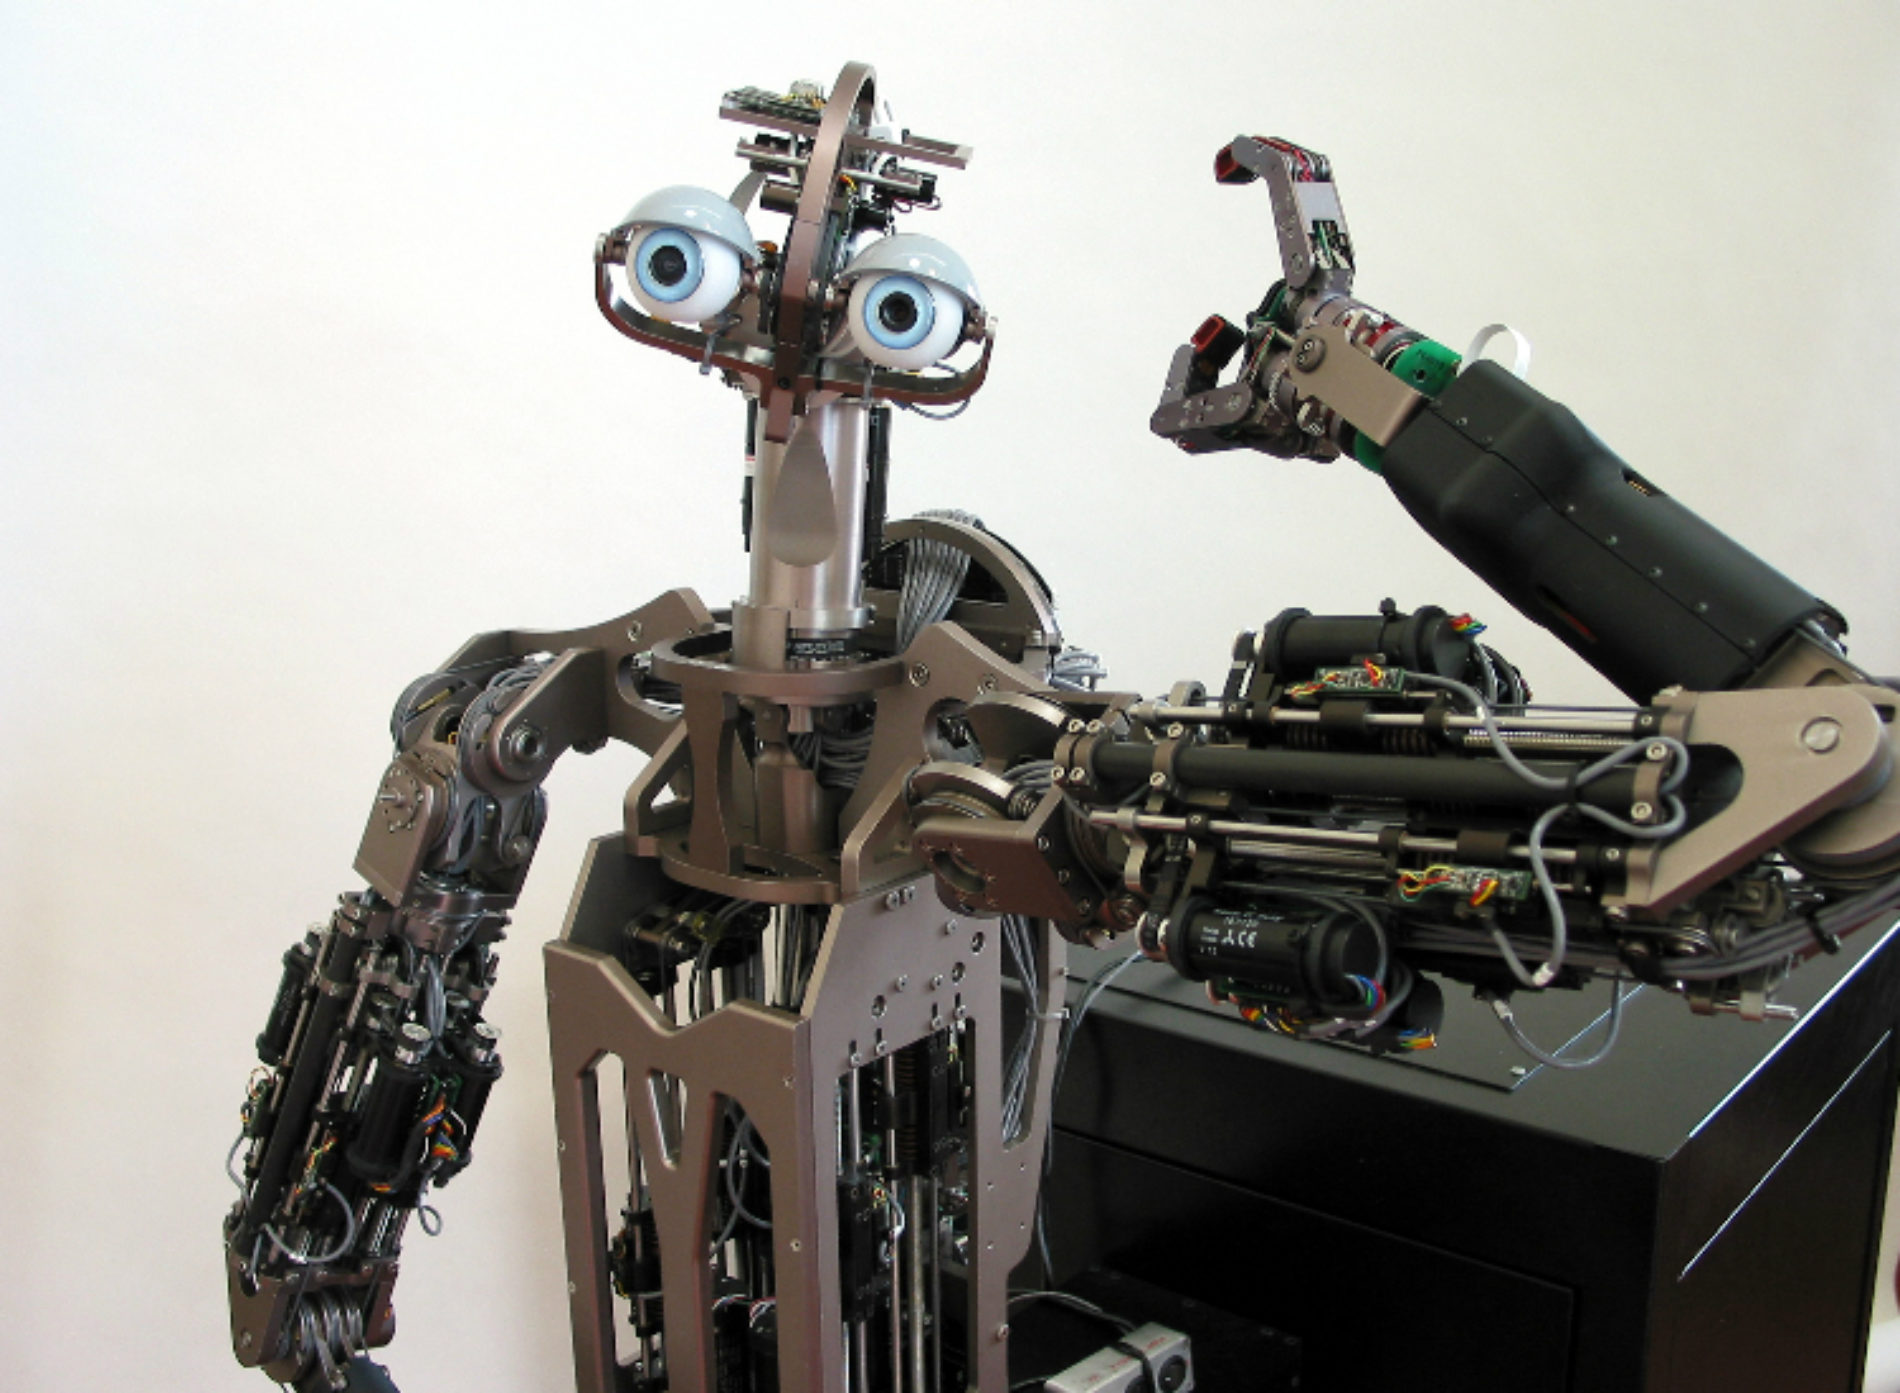
\includegraphics[width=0.6\linewidth]{tex/figs/domo-foto.jpg}
    \caption{Foto Robô Domo (Fonte: http://www.robotsvoice.com)}
    \label{fig:domorobot}
\end{figure}

Este projeto teve particular importância pois muitos dos conceitos explorados vieram a compor patentes e futuramente partes dos robôs Baxter e Meka, respectivamente das empresas Rethink Robotics e Meka Robótics. Da mesma equipe que desenvolveu o Domo surgiu a Meka Robótics a partir de Aaron Singer e Jeff Weber. E dos trabalhos de Pratt e Williason \cite{pratt1995series} surgiu a empresa Rethink Robotics fundada por Rodney Brooks, então professor do MIT em 1995.

% Baxter vs Meka
Embora com design completamente diferente, ambos robôs incorporam o uso atuadores série elásticos em cada uma das juntas como elemento de segurança. Desta forma qualquer pessoa pode manusear os braços de ambos robôs de maneira livre. No entanto este sistema também confere ao robô uma maior suscetibilidade a influência de outros estímulos externos como a ação da gravidade na dinâmica do robô tornado necessária o uso de soluções de controle complementares para garantir a precisão. \cite{nobody} Este problema é resolvido de forma diferente em cada uma das plataformas. No Baxter a compensação da gravidade é feita de forma completamente mecânica por uma série de molas \cite{nobody}, o que em parte explica seu maior tamanho. E no Meka esta é feita via software através do modelo dinâmico em conjunto da biblioteca KDL \cite{nobody}, conferindo um design mais compacto. 

% Robonauta -> Paradigmas atuais

\section{Definição do problema}

No Laboratório de Automação e Robótica ( LARA - UnB ) encontra-se disponível o braço robótico Meka A2 fornecido pela Meka Robotics. Daqui em diante será denominado apenas Meka. O Meka é um braço complacente antropomórfico composto por 7 juntas e uma garra desenvolvido para pesquisas na área de interação com pessoas. Cada uma das juntas possui um atuador série elástico composto de um motor sem escova e um redução mecânica por onda de deformação.

Em trabalhos anteriores foi observado um desempenho ineficiente nos controles cinemáticos implementados em contraste ao resultado observado em outras plataformas robóticas e em simulação. Tal arquitetura não encontra-se devidamente documentada e detalhada. Desta forma, neste trabalho, propõe-se realizar uma caracterização mais detalhada desta arquitetura de controle para compreender sua implicação no desempenho dos controles cinemáticos testados e propor melhorias que resultem em trajetórias mais precisas levando em conta as características próprias do sistema.

\section{Metodologia}

% Rever completamente
Este trabalho foi desenvolvido em três etapas: estudo sobre teoria clássica de controle de manipuladores, revisão e acompanhamento de trabalhos anteriores feitos no LARA utilizando o Meka e por fim a investigação e experimentação usando a plataforma. Esta investigação foi feita a partir da métodos científicos de análise e síntese do processo. Por meio da análise foram estudados cada um dos componentes utilizados tanto de hardware como software em seu detalhes. E contraponto foi alguns dos fenômenos foram sintetizados por meio de simulações visando ampliar a compreensão de quais fatores ocasionam ao Meka um desempenho inferior outros braços robóticos avaliados pelos trabalhos de Murilo \cite{nobody} e Marcos \cite{nobody}.

\subsection{Estudo controle de manipuladores}

Inicialmente foi feito um estudo sobre a teoria clássica do controle cinemático e dinâmico de manipuladores incluindo a representação por cadeia cinemática usando matrizes homogenias e a simplificação através da notação de Denavit-Hatemberg.

\subsection{Revisão trabalhos anteriores}

Inicialmente foi feito um estudo sobre os trabalho anteriores desenvolvidos na plataforma no Laboratório de Automação e Robótica ( LARA - UnB ) bem como estratégias clássicas no controle de robôs industriais. Alguns destes trabalhos puderam ser acompanhados ao longo da execução como o caso dos trabalhos desenvolvidos por Marcos Pereira e pelo Rafael Koji de modo a facilitar a transmissão do conhecimento relacionado as contribuições de cada um ao projeto bem como presenciar as dificuldades relacionadas ao controle do braço robótico.

\subsection{Investigação e experimentação a partir da plataforma}

Após o estudo preliminar foi adotado uma metodologia de investigação baseada em ciclos compostos por 3 etapas, descritas a seguir. Estas etapas são baseadas nos princípios de desenvolvimento ágil \ref{noref} e têm como objetivo acelerar e otimizar os esforços.

% TODO Colocar Referência

% Diagrama das etapas
\begin{enumerate}
    \item Análise e Formulação de Hipóteses
    \item Formulação de Testes para as Hipóteses
    \item Avaliação de Hipóteses ( Testes Experimentais e Estudo teórico )
\end{enumerate}

Cada ciclo possui duração variável de acordo com o nível de aprofundamento necessário para satisfazer os objetivos levantados para cada momento do projeto. O objetivo central é ao final de um ciclo é trazer algum aprimoramento quanto ao entendimento do sistema ou ainda quanto ao comportamento final na realização da tarefa.

No inicio de cada ciclo é feito um estudo do sistema através da modelagem do sistema e da definição de uma métrica para avaliar o comportamento. Então o comportamento do sistema real é comparado com o modelo adotado e as expectativas de comportamento. Os objetivos são traduzidos em uma métrica, compondo um conjunto de indicadores que permita avaliar se tarefa foi executada e como foi o processo de execução. A cada novo aspecto avaliado podem ser introduzidos novos indicadores em conjunto aos antigos ou modificados. 

Com base nisto são levantadas hipóteses quanto ao comportamento quanto ao fato de satisfazer ou não o modelo adotado e possíveis condutas para aprimorar os resultados dentro da métrica proposta. Para cada uma destas condutas é levantado um teste de verificação que pode incluir consulta bibliográfica, simulações a partir do modelo e experimentos com o Meka. Os resultados desta etapa são então levados para a etapa de observação e confrontados novamente e assim o ciclo se repete.

Resultados positivos são incorporados e resultados negativos avaliados quanto a possíveis correções. Tudo é registrado para permitir futuras avaliações. O resultado de cada dia foi feito um registro das atividades e todo material produzido foi colocado no GitHub \footnote{www.github.com/lara-unb/Meka} de forma a permitir o uso futuro na validação do comportamento após modificações futuras.

\section{Estrutura do Documento}

Este trabalho está dividido em 5 capítulos visando facilitar o entendimento. Estes estão organizados da seguinte forma:

\begin{itemize}
    \item \textit{Cap. \ref{ch:intro} Introdução} : Breve Apresentação e Histórico sobre Robótica Colaborativa.
    \item \textit{Cap. \ref{ch:teory-reference} Fundamentos} : Conceitos teóricos e tecnologias usadas no trabalho.
    \item \textit{Cap. \ref{ch:develop} Desenvolvimento} : Metodologia usada na investigação dos problemas e análise dos dados.
    \item \textit{Cap. \ref{ch:results} Resultados} : Dados obtidos ao longo do trabalho.
    \item \textit{Cap. \ref{ch:conclusoes} Conclusão} : Resultado final do trabalho e propostas de trabalhos futuros.
\end{itemize}


\begin{comment}
Fundamentos
\end{comment}
\chapter{Fundamentos\label{chap:FundamentacaoMatematica}}

% Resumo opcional. Comentar se não usar.
\resumodocapitulo{Resumo opcional.}


\section{Introdução}

Introduzir.


\begin{comment}
Conclusões
\end{comment}
\chapter{Conclusão} \label{ch:conclusoes}

\section{Perspectivas Futuras}

% Introdução 
% - Cobots
Neste trabalho foi apresentado um detalhamento maior da arquitetura de controle implementada no Meka permitindo conhecer os fundamentos das tecnologias envolvidas no desenvolvimento de manipuladores robóticos cooperativos bem como vivenciar os principais desafios em manter um manipulador robótico seguro e um desempenho razoável na execução de alguma tarefa. Foi buscado ir a origem inicial de cada problema, tanto do ponto de vista histórico como de cada componente utilizado. O redução no preço dos computadores, o uso de sistemas série elásticos para controle preciso de torque e bem como a disponibilidade de soluções open-source entre outras tecnologias permitiram que manipuladores robóticos pudessem alcançar mais pessoas. Soluções robóticas sempre estiveram no plano de tecnologias de alto padrão e distantes da realidade da maioria porém têm sido crescente os esforços na difusão.

% Fundamentação
% - Qualidade do HW
O Meka foi implementado com componentes de alto desempenho seguindo a filosofia do mercado na sua época de lançamento. Embora hoje, outras tecnologias estão sendo incorporadas ao projeto de robôs complacentes como o uso de sistemas freios, esta plataforma ainda representa uma ótima plataforma para o estudo de controladores dinâmicos bem como cada uma dos componentes envolvidos. Como exemplo, o uso de atuadores série elásticos, embora estejam implementados no Meka com motores e sistemas de transmissão de ponta, podem também ser incorporados em outros projetos como solução aos problemas de instabilidade do controle na interação com superfícies rígidas em aplicações para locomoção. Ou ainda em aplicação de forças na área de fisioterapia.

% Desenvolvimento
No que tange ao sistema de controle implementado, foi percebido que nos trabalhos anteriores foi alcançado o limite de desempenho dos controladores de baixo atuais do sistema M3. No entanto, dado que o sistema de controle é completamente open-source e possui um sistema embarcado capaz de uma desempenho maior ainda existe um enorme potencial que pode ser explorado para uso em trabalhos futuros. Uma vez que as soluções implementadas incorporam técnicas de filtragem e controle dinâmico que podem ser aprimoradas.

% Resultados
% - Juntas
Os controladores de posição de juntas foram ajustados para responderem de forma similar para todas as juntas. Embora esta seja uma estratégia que permite que a resposta controle seja similar e facilite a avaliação dos controladores cinemáticos, na prática o comportamento o comportamento de cada junta é bem diferente. Para um ganho de desempenho, pode ser explorado a possibilidade de controladores ajustados para respostas diferente para cada uma das juntas. Em conjunto com as características particulares da geometria do braço, um desempenho melhor pode ser atingido, por permitir as juntas do ombro operarem com uma resposta mais rápida.

A técnica atualmente implementada para compensação da gravidade usa apenas a posição das juntas para uma gerar um torque em feedforward a partir do modelo cinemático e dinâmico do robô. Outras técnicas podem ser utilizadas para que as velocidade final e o torque possam também ajustadas. Também foi notado que o acoplamento entre a posição e a orientação introduzido por quatérnions duais pode ser explorado a partir das características das juntas do robô, uma vez que a composição do ombro e do pulso podem atuar como dois guibal em oposição permitindo um estudo maior da dinâmica da rotação no movimento do efetuador.

% Trabalhos Futuros Controle + Metodologia
Para trabalhos futuros na plataforma é sugerido a identificação do modelo dos atuadores série elástico disponíveis na plataforma visando a implementação de um controle de juntas mais preciso. No intuito de apresentar a modelagem completa do braço, uma vez que esta não está disponível. Também é apresentado a possibilidade de estudo em controle multivariado a partir de espaço de estados para permitir explorar os efeitos das não linearidade em composição com o modelo cinemático do robô, gerando uma solução que controle ao mesmo a cinemática e dinâmica do movimento. Os conceitos implementados na plataforma podem também compor partes de outros projetos com explorado por outras universidades que passaram a produzir seus próprios atuadores, braços e plataformas robóticas.

%Com base nos resultados obtidos, observou-se o controle implementado em ROS está sendo executado com um frequência maior que a resposta das camadas inferiores subsequentes de controle. Este fator pode estar causando uma instabilidade no controle, uma vez que o erro acumulado durante o tempo que o robô permanece parado até o ocorrer a resposta é compensado com um esforço maior de controle, percebido nos registros dos experimentos como saltos periódicos na velocidade. Estes efeitos eram percebidos com maior nitidez no eixo vertical, uma vez que a maior perturbação ao sistema se dava pelo efeito da ação do campo gravitacional.

%Como proposta, serão efetuados ao longo do trabalho a continuidade do estudo da plataforma em conjunto com a identificação da planta completa. Por se tratar de um sistema complexo que envolve diversos sub-sistemas atuando em conjunto, este estudo será pautado as principais influências de cada componente no controle final da posição do efetuador.

%Também serão analisado um comparativo das estratégias de controle por velocidade e por posição a partir da descrição cinemática implementada em Quatérnions Duais. O controle por velocidade apresenta uma resposta mais rápida que os controles de velocidade por retirar a necessidade e esperar a posição final ser atingida e eliminaria a necessidade do passo de integração por parte de alguns dos controladores implementados. Ao passo que poderia permitir o uso direto de controladores mais baixos, uma vez que os motores Brushless possuem os controle de torque e velocidade que são convertidos em posição por meio da placa DSP.

%Ao final, o objetivo é trazer desempenho melhor em termos de precisão no controle do Meka e facilitar o uso deste no laboratório em projetos futuros por meio do aprofundamento na documentação e estudo iniciados em trabalhos anteriores. Em conjunto é apresentado um detalhamento das sistemas empregados para inspirar o uso em projetos futuros de sistemas robóticos desenvolvidos pelo laboratório, uma vez soluções similares baseadas em atuadores série elásticos estão presentes muitos projetos recentes.

\begin{comment}
Bibliografia
\end{comment}


\renewcommand{\bibname}{REFERÊNCIAS BIBLIOGRÁFICAS}
\addcontentsline{toc}{chapter}{REFERÊNCIAS BIBLIOGRÁFICAS}

\bibliographystyle{abnt-num}
\bibliography{bibliography}


\begin{comment}
Anexos
\end{comment}


\anexos
\makeatletter
% não retirar estes comandos
\renewcommand{\@makechapterhead}[1]{%
  {\parindent \z@ \raggedleft \setfontarial\bfseries
\LARGE \thechapter. \space\space
\uppercase{#1}\par
\vskip 40\p@
}
}
\makeatother

\begin{comment}
Anexo I: Descrição do CD
\end{comment}


\chapter{Descrição do conteúdo do CD}

\label{AnCD}

Descrever CD.


\refstepcounter{noAnexo}

\begin{comment}
Anexo II: Programas Utilizados
\end{comment}


\chapter{Programas utilizados}

Quais programas foram utilizados?


\refstepcounter{noAnexo}

\begin{comment}
Acrescente mais anexos conforme julgar necessário.
\end{comment}

\end{document}
